\documentclass{bredelebeamer}

%%%%%%%%%%%%%%%%%%%%%%%%%%%%%%%%%%%%%%%%%%%%%%%%

\title[Programación en MatLAB]{Introducción a la programación con MatLAB}
\subtitle{Módulo 05 - Gráficos en matlab}

\author{- AUTORES - \inst{1}}
\institute[UNIVERSIDAD]
{
  \inst{1}%
  - NOMBRE UNIVERSIDAD - 
  }

\date{AÑO}

\subject{Taller de programación}

\logo{

\includegraphics[scale=0.15]{images/logo.png}
}

%%%%%%%%%%%%%%%%%%%%%%%%%%%%%%%%%%%%%%%%%%%%%%%%%%%%%%%%%%%%%%%%%%%%%
\begin{document}

\begin{frame}
  \titlepage 
\end{frame}

%%%%%%%%%%%%%%%%%%%%%%%%%%%%%%%%%%%%%%%%%%%%%%%%%%%%%%%%%%%%%%%%%%%%%

% Sección de graficación

%%%%%%%%%%%%%%%%%%%%%%%%%%%%%%%%%%%%%%%%%%%%%%%%%%%%%%%%%%%%%%%%%%%%%

\section{Graficación}

\begin{frame}{Primeros Conceptos}
Ej. Ejecute el siguiente código. Obtener conclusiones.
\lstinputlisting[xleftmargin=.1\textwidth]{scripts/ej1.m}
\begin{exampleblock}{Comando}
Ver comando: \textbf{plot(x,y)}
\end{exampleblock}
\end{frame}

\begin{frame}{Primeros Conceptos}
\begin{center}
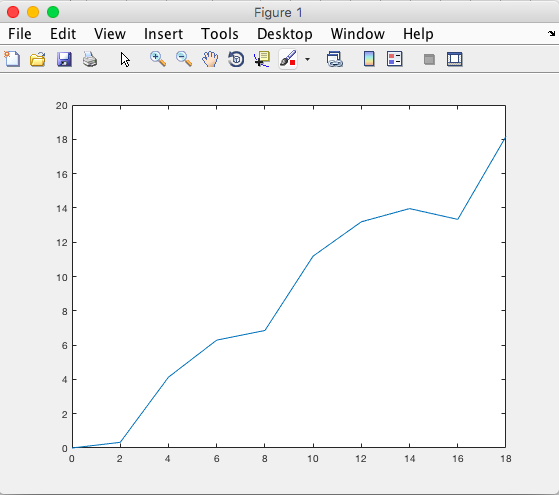
\includegraphics[scale=0.35]{images/pantalla14.png}
\end{center}
\end{frame}

\begin{frame}{Títulos, etiquetas y grilla}
\begin{exampleblock}{Comando}
Ver comando: \textbf{title('Inserte título')}
\end{exampleblock}
\begin{exampleblock}{Comando}
Ver comando: \textbf{xlabel('Inserte etiqueta eje x')}
\end{exampleblock}
\begin{exampleblock}{Comando}
Ver comando: \textbf{ylabel('Inserte etiqueta eje y')}
\end{exampleblock}
\begin{exampleblock}{Comando}
Ver comando: \textbf{grid on / grid off}
\end{exampleblock}
\end{frame}

\begin{frame}{Títulos, etiquetas y grilla}
Ej. Ejecute el siguiente código. Obtener conclusiones.
\lstinputlisting[xleftmargin=.1\textwidth]{scripts/ej2.m}
\end{frame}

\begin{frame}{Títulos, etiquetas y grilla}
\begin{center}
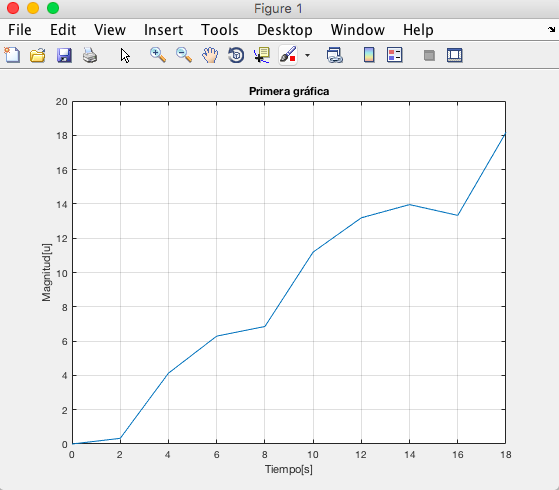
\includegraphics[scale=0.35]{images/pantalla15.png}
\end{center}
\end{frame}

\begin{frame}{Títulos, etiquetas y grilla}
\begin{alertblock}{Tener en cuenta}
Se debe crear una gráfica antes de agregarle título y etiquetas. Si primero se especifica el título y las etiquetas, se borrarán cuando se ejecute el comando plot.
\end{alertblock}
\end{frame}

\begin{frame}{Gráficos múltiples}
Ej. Ejecute el siguiente código. Obtener conclusiones.
\lstinputlisting[xleftmargin=.1\textwidth]{scripts/ej3.m}
\end{frame}

\begin{frame}{Gráficos múltiples}
Ej. Ejecute el siguiente código. Obtener conclusiones.
\lstinputlisting[xleftmargin=.1\textwidth]{scripts/ej3.m}
\begin{exampleblock}{Comando}
Ver comandos:\\ \textbf{figure(numero)}\\ \textbf{figure('name','figura de ejemplo')}
\end{exampleblock}
\end{frame}

\begin{frame}{Gráficos múltiples}
Ej. Ejecute el siguiente código. Obtener conclusiones.
\lstinputlisting[xleftmargin=.1\textwidth]{scripts/ej4.m}
\begin{exampleblock}{Comando}
Ver comando: \textbf{hold on / hold off}
\end{exampleblock}
\end{frame}

\begin{frame}{Gráficos múltiples}
\begin{center}
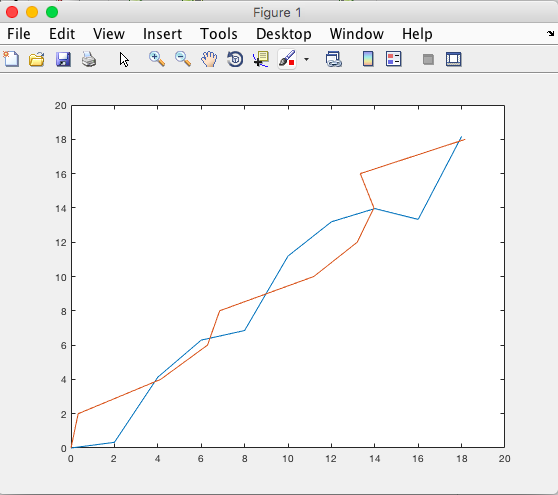
\includegraphics[scale=0.35]{images/pantalla16.png}
\end{center}
\end{frame}

\begin{frame}{Estílos de líneas}
Matlab permite aplicar distintos estílos a las gráficas, entre las cuales se tienen:
\begin{itemize}
\item Estílos de línea: sólido, rayado, punteado y raya-puto
\item Tipos de punto: estrellas, círculos, marcas con x, entre otros
\item Opciones de color: azul, verde, rojo, entre otros
\end{itemize}
\end{frame}

\begin{frame}{Estílos de líneas}
\begin{table}[]
\centering
\begin{tabular}{|c|c|c|c|c|c|}
\hline
Línea      & Indicador & Punto          & Indicador       & Color           & Indicador      \\ \hline
sólida     & -         & punto          & .               & azul            & b              \\ \hline
punteada   & :         & círculo        & o               & verde           & g              \\ \hline
raya-punto & -.        & marca x        & x               & rojo            & r              \\ \hline
rayada     & --        & más            & +               & cian            & c              \\ \hline
           &           & estrella       & *               & magenta         & m              \\ \hline
           &           & cuadrado       & s               & amarrillo       & y              \\ \hline
           &           & diamante       & d               & negro           & k              \\ \hline
           &           & \multicolumn{2}{c|}{entre otros} & \multicolumn{2}{c|}{entre otros} \\ \hline
\end{tabular}
\end{table}
\begin{exampleblock}{Comando}
Ver comando: \textbf{plot(x,y,'características')}
\end{exampleblock}
\end{frame}

\begin{frame}{Estílos de líneas}
\begin{center}
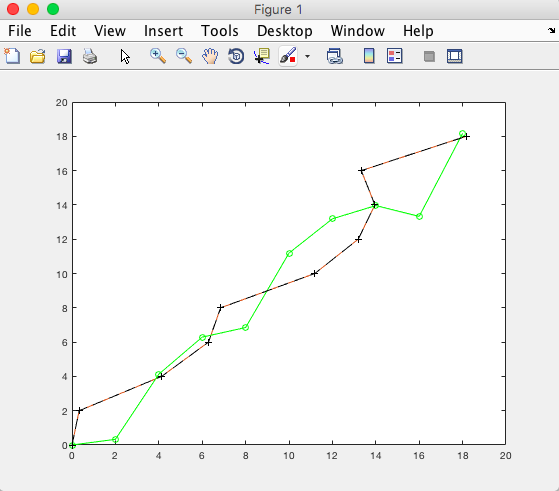
\includegraphics[scale=0.35]{images/pantalla17.png}
\end{center}
\end{frame}

\begin{frame}{Escalamiento y leyendas}
Escalamiento:\\
\begin{exampleblock}{Comando}
Ver comando: \textbf{axis([xmin xmax ymin ymax zmin zmax])}
\end{exampleblock}
\begin{exampleblock}{Comando}
Ver comando: \textbf{axis()}
\end{exampleblock}
\end{frame}

\begin{frame}{Escalamiento y leyendas}
Escalamiento:\\
\begin{exampleblock}{Comando}
Ver comando: \textbf{axis([xmin xmax ymin ymax zmin zmax])}
\end{exampleblock}
\begin{exampleblock}{Comando}
Ver comando: \textbf{axis()}
\end{exampleblock}
\begin{alertblock}{Tener en cuenta}
Matlab selecciona automáticamente escalamientos adecuados en los ejes x y y de no ser especificados.
\end{alertblock}
\end{frame}

\begin{frame}{Escalamiento y leyendas}
Leyendas:\\
\begin{exampleblock}{Comando}
Ver comando: \textbf{legend('etiqueta1','etiqueta2')}
\end{exampleblock}
\end{frame}

\begin{frame}{Escalamiento y leyendas}
\begin{center}
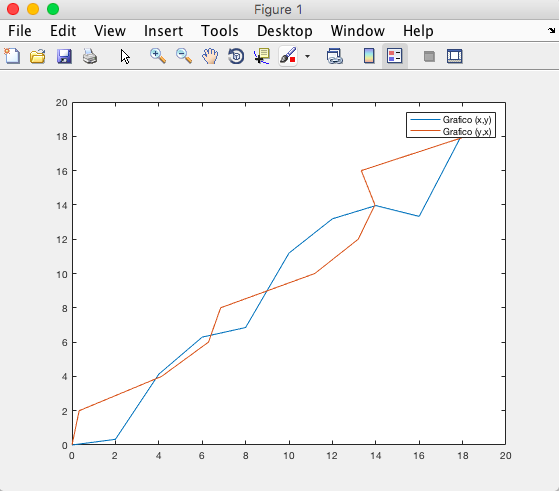
\includegraphics[scale=0.35]{images/pantalla18.png}
\end{center}
\end{frame}

\begin{frame}{Escalamiento y leyendas}
Texto:\\
\begin{exampleblock}{Comando}
Ver comando: \textbf{text(coordenada X, coordenada Y, 'texto')}
\end{exampleblock}
\end{frame}

\begin{frame}{Escalamiento y leyendas}
\begin{center}
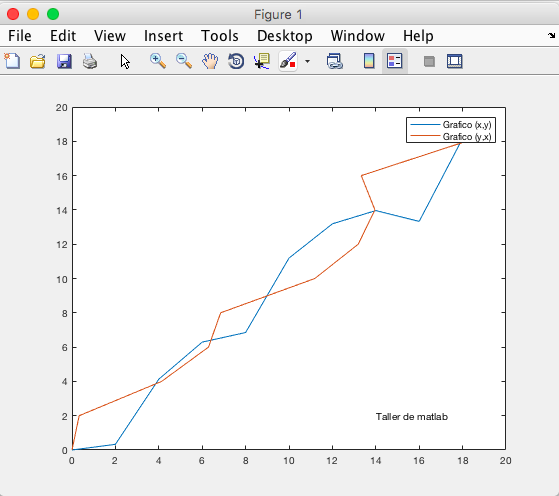
\includegraphics[scale=0.35]{images/pantalla19.png}
\end{center}
\end{frame}

\begin{frame}{Ejercicio práctico 6}
\begin{enumerate}
\item Grafique x contra y para y = sen(x). Sea x que varía desde 0 hasta 2pi en incrementos de 0.1pi
\item Agregue un título y etiqueta a su gráfica
\item Grafique x contra $y_1$ y $y_2$ para $y_1 = sen(x)$ y $y_2 = cos(x)$. Sea x que varía desde 0 hasta 2pi en incrementos de 0.1pi. Agregue un título y etiqueta a su gráfica.
\item Vuelva a crear la gráfica de la parte 3, pero haga la línea sen(x) rayada y roja. Haga la línea cos(x) verde y punteada.
\item Agregue una leyenda a la gráfica de la parte 4.
\item Ajuste los ejes de modo que el eje x vaya de -1 a 2pi+1 y el eje y de -1.5 a + 1.5.
\end{enumerate}
\begin{block}{Sugerencia}
Para limpiar una figura, use el comando clf. Para cerrar una ventana de figura, use el comando close.
\end{block}
\end{frame}

\begin{frame}{Subgráficas}
La subdivisión de una ventana (figura) se realiza con el comando subplot
\begin{exampleblock}{Comando}
Ver comando: \textbf{subplot(Mfilas,Ncolumnas,posición)}
\end{exampleblock}
\end{frame}

\begin{frame}{Subgráficas}
Ej. Ejecutar las siguiente líneas. Obtener conclusiones.
\lstinputlisting[xleftmargin=.2\textwidth]{scripts/ej5.m}
\end{frame}

\begin{frame}{Subgráficas}
\begin{center}
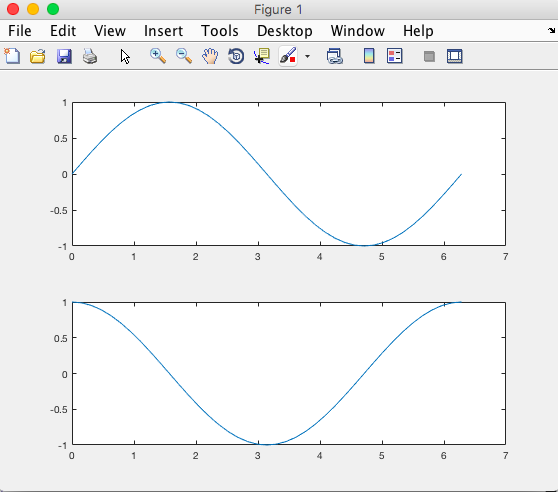
\includegraphics[scale=0.35]{images/pantalla20.png}
\end{center}
\end{frame}

\begin{frame}{Subgráficas}
Ej. Ejecutar las siguiente líneas. Obtener conclusiones.
\lstinputlisting[xleftmargin=.2\textwidth]{scripts/ej6.m}
\end{frame}

\begin{frame}{Subgráficas}
\begin{center}
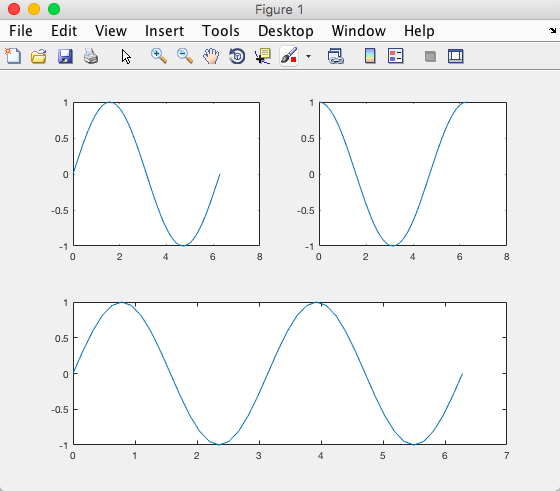
\includegraphics[scale=0.35]{images/pantalla21.png}
\end{center}
\end{frame}

\begin{frame}{Subgráficas}
\begin{center}
Procesamiento de una señal de ECG
\end{center}
\begin{center}

\includegraphics[scale=0.35]{images/img43.png}
\end{center}
\end{frame}

\begin{frame}{Ejercicio práctico 7}
\begin{enumerate}
\item Subdivida una ventana de figura en dos filas y una columna.
\item En la ventana superior, grafique $y=tan(x)$ para $-1.5<=x,<= +1.5$. Use un incremento de 0.1.
\item Agregue un título y etiqueta de eje a su gráfica.
\item En la ventana inferior, grafique $y=senh(x)$ para el mismo rango.
\item Agregue un título y etiquetas a su gráfica.
\item Intente de nuevo los ejercicios anteriores, pero divida la ventana de figura verticalmente en lugar de horizontalmente.
\end{enumerate}
\end{frame}

\begin{frame}{Otros tipos de gráfica}
Matlab permite hacer otros tipos de gráficos 2D, por ejemplo:
\begin{itemize}
\item Gráficos polares
\item Gráficos Logarítmicos
\item Gráficos de barra
\item Gráficos de pastel
\item Histogramas
\item Gráficos de error
\end{itemize}
\end{frame}

\begin{frame}{Otros tipos de gráfica}
Gráficos polares
\begin{exampleblock}{Comando}
Ver comando: \textbf{polar(theta,r)}
\end{exampleblock}
\begin{columns}
\begin{column}{0.5\textwidth}
\lstinputlisting[xleftmargin=.2\textwidth]{scripts/ej7.m}
\end{column}
\begin{column}{0.5\textwidth}
\begin{center}
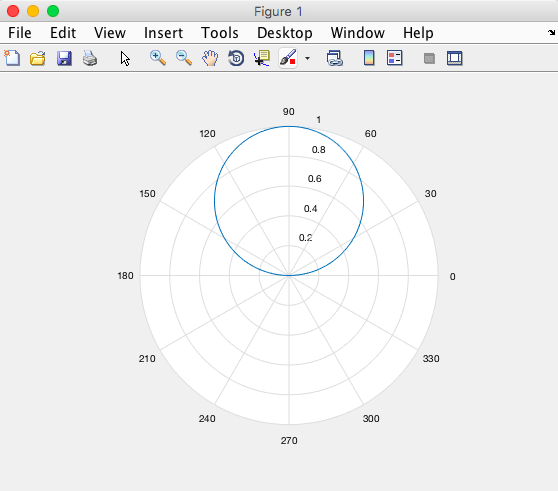
\includegraphics[scale=0.2]{images/pantalla22.png}
\end{center}
\end{column}
\end{columns}
\end{frame}

\begin{frame}{Otros tipos de gráfica}
Gráficos logarítmicos
\begin{exampleblock}{Comando}
Ver comando: \textbf{$semilogx(x,y)$}\\
Ver comando: \textbf{$semilogy(x,y)$}\\
Ver comando: \textbf{$loglog(x,y)$}
\end{exampleblock}
\begin{columns}
\begin{column}{0.5\textwidth}
\lstinputlisting[xleftmargin=.2\textwidth]{scripts/ej8.m}
\end{column}
\begin{column}{0.5\textwidth}
\begin{center}
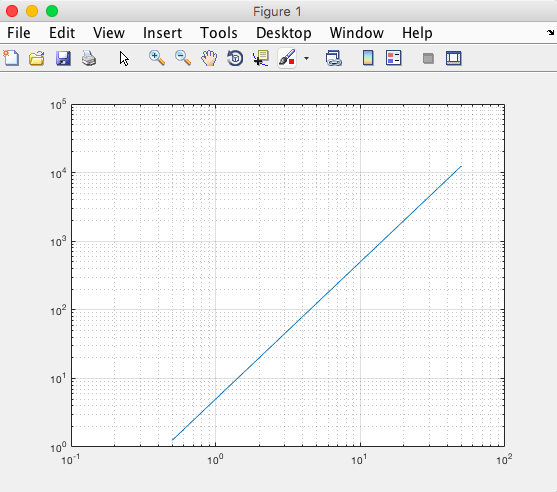
\includegraphics[scale=0.2]{images/pantalla23.png}
\end{center}
\end{column}
\end{columns}
\end{frame}

\begin{frame}{Otros tipos de gráfica}
\begin{center}
Filtro pasa bajos
\end{center}
\begin{center}

\includegraphics[scale=0.5]{images/img41.png}
\end{center}
\end{frame}

\begin{frame}{Otros tipos de gráfica}
Gráficos de barra
\begin{exampleblock}{Comando}
Ver comando: \textbf{$bar(x)$}\\
Ver comando: \textbf{$bar3(x)$}\\
\end{exampleblock}
\begin{columns}
\begin{column}{0.5\textwidth}
\lstinputlisting[xleftmargin=.2\textwidth]{scripts/ej9.m}
\end{column}
\begin{column}{0.5\textwidth}
\begin{center}
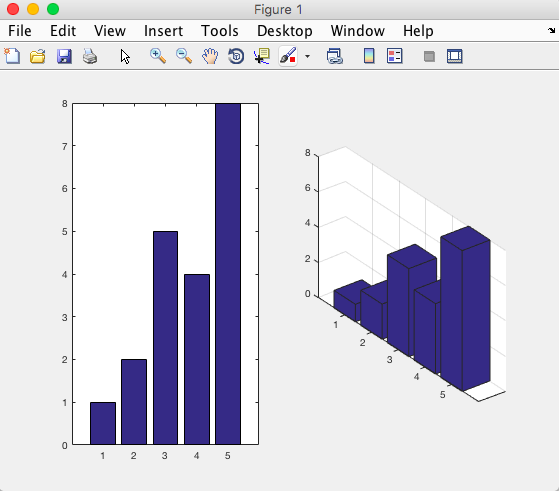
\includegraphics[scale=0.2]{images/pantalla24.png}
\end{center}
\end{column}
\end{columns}
\end{frame}

\begin{frame}{Otros tipos de gráfica}
\begin{center}
Asistencia a cines en Colombia
\end{center}
\begin{center}

\includegraphics[scale=0.5]{images/img42.png}
\end{center}
\end{frame}

\begin{frame}{Otros tipos de gráfica}
Gráficos de pastel
\begin{exampleblock}{Comando}
Ver comando: \textbf{$pie(x)$}\\
Ver comando: \textbf{$pie3(x)$}\\
\end{exampleblock}
\begin{columns}
\begin{column}{0.5\textwidth}
\lstinputlisting[xleftmargin=.2\textwidth]{scripts/ej10.m}
\end{column}
\begin{column}{0.5\textwidth}
\begin{center}
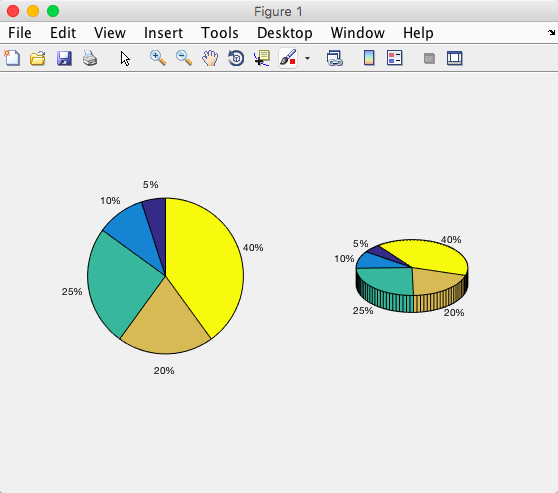
\includegraphics[scale=0.2]{images/pantalla25.png}
\end{center}
\end{column}
\end{columns}
\end{frame}

\begin{frame}{Otros tipos de gráfica}
Histogramas
\begin{exampleblock}{Comando}
Ver comando: \textbf{hist(x)}
\end{exampleblock}
\begin{columns}
\begin{column}{0.5\textwidth}
\lstinputlisting[xleftmargin=.2\textwidth]{scripts/ej11.m}
\end{column}
\begin{column}{0.5\textwidth}
\begin{center}
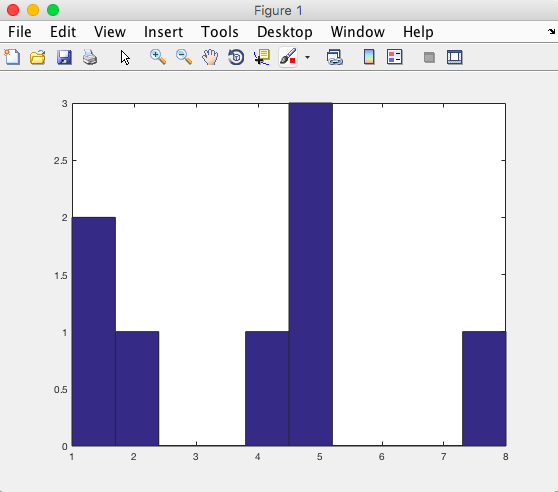
\includegraphics[scale=0.2]{images/pantalla26.png}
\end{center}
\end{column}
\end{columns}
\end{frame}



\begin{frame}{Otros tipos de gráfica}
\begin{center}
Ecualización de Histograma
\end{center}
\begin{center}

\includegraphics[scale=0.5]{images/img40.png}
\end{center}
\end{frame}

\begin{frame}{Otros tipos de gráfica}
Graficos de error
\begin{exampleblock}{Comando}
Ver comando: \textbf{errorbar(x,y,e)}
\end{exampleblock}
\begin{columns}
\begin{column}{0.5\textwidth}
\lstinputlisting[xleftmargin=.2\textwidth]{scripts/ej12.m}
\end{column}
\begin{column}{0.5\textwidth}
\begin{center}
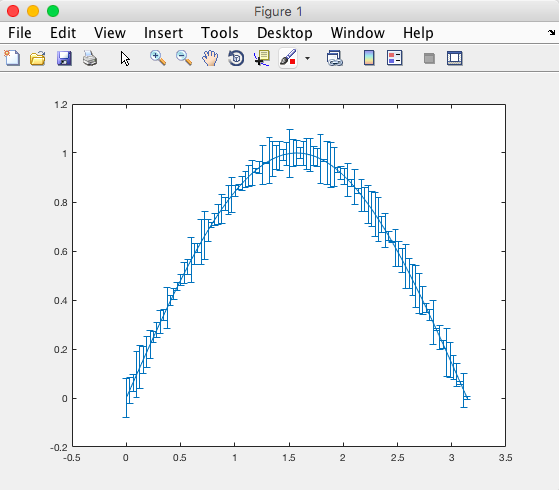
\includegraphics[scale=0.2]{images/pantalla27.png}
\end{center}
\end{column}
\end{columns}
\end{frame}

\end{document}
